%
% Categorifying the zx-calculus
% Introduction
% arXiv v2
%

\documentclass[./Catfying_zxCalc--Master.tex]{subfiles} % ./mainfilename.tex

\input{Catfying_zxCalc--Preamble.tex}
\addbibresource{Catfying_zxCalc--Bibliography.bib}

%%%%%%%%%%%%%%%%%%
%%%%%%%%%%%%%%%%%%
% 
\begin{document}
%
%%%%%%%%%%%%%%%%%%
%%%%%%%%%%%%%%%%%%

%%%%%%%%%%%%%
% INTRODUCTION
\section{Introduction}
\label{sec:Introduction}
%%%%%%%%%%%%%

Compositionality is becoming increasingly recognized as a viable method to model complex systems such as those found in 
physics \cite{AbramCoecke_CatSemanticQuantum}, 
computer science \cite{SassoneSobocinski_PetriNets}, 
and biology \cite{BaezFongPollard_CompMarkovProcesses}.  
The idea is to study smaller, simpler systems and ways of connecting them together.  The word \emph{compositionality} suggests that category theory can play a key role, and indeed it does.  Systems are morphisms and connections are morphism composition.   

While studying compositionality, one commonly sees the use of diagrams and diagrammatic calculi. The example at hand here is the zx-calculus.  The advantage of working with diagrams is that it provides a user with an intuitive syntax in which to reason with.  Such diagrams are typically made from graphs or topological strings.  Occasionally, additional data is attached to nodes, edges, or strings as needed. One such instance is open Markov chains
\cite{Pollard_OpenMarkov}. 
These use graphs whose nodes are labeled with an integer valued `population' and edges by a non-negative value describing the rate at which residents of the source node move to the target node. 

Another common component of diagrammatic calculi is the notion of equality between diagrams.  Often, as in the present case, equality is presented as a relation derived from some collection of \emph{rewrite rules}. That is, we say that a diagram $D$ can be rewritten to diagram $D'$ if there is a rule allowing us to do so.  Because we are currently only interested in symmetric rewrite rules, these rewrite rules generate an equivalence relation which we take to mean equality. 

The author is part of a larger project whose goal is to find a common framework in which to study diagrammatic calculi, in particular those whose diagrams have a notion of \emph{input} and \emph{output}. We start with the several observations. At this time, diagrammatic calculi are typically discussed in the context of 1-categories, where the diagrams form the morphisms and composition is by `gluing' diagrams along coinciding inputs and outputs. Diagrams are identified by rewrite rules as mentioned above. Though, with this perspective, the information contained in a rewrite rule is squashed down to a mere proposition, in the type theoretic sense. We believe that, morally, rewrite rules ought to not be squashed. They should be fully contained in the syntactic structure. The way we do this is by including them as 2-cells in a bicategory.  

What should such a bicategory look like? We continue to think of diagrams as morphisms. Because we want to connect (that is, compose) a pair of diagrams $D$, $D'$ when the inputs of $D$ match the outputs of $D'$, the 0-cells of our bicategory should provide a way to do so.  The most obvious method would be to take sets as 0-cells, then a 1-cell $D \from x \to y$ is a diagram whose set of inputs is $x$ and set of outputs is $y$. The upper layer, our 2-cells, consists of rewrite rules $r \from D \to D'$.  This is a rough sketch, of course, to which we now add a bit more detail.

It is helpful to consider a hypothetical system modeled by a directed graph $D$. Suppose that we would like $D$ to have inputs $I$ and outputs $O$, each subsets of the $D$-nodes.  We can build this information into a cospan $I \to D \to O$, where $I$ and $O$ are considered as edgeless graphs and arrows as graph morphisms.  This is a 1-cell.  To include rewrite rules into the picture, we use the notion of \emph{double pushout rewriting}
\cite{Corradini_AlgApprGraphTrans} 
which encodes a rewrite rule from, say graphs, $D$ to $D'$ as a span of graphs $D \gets K \to D'$. Now 2-cells, which capture the rewrite rules, are isomorphism classes of spans of cospans as depicted in Figure \ref{fig:spans of cospans}.  

That we have actually described a bicategory was proved by the author \cite{Cicala_SpansCospans}.  The proof started with a topos $T$ and constructed a bicategory $\bimonspcsp{T}$ with $T$-objects as 0-cells, $T$-cospans as 1-cells, and isomorphism classes of $T$-spans of cospans whose span legs are $T$-monomorphisms as 2-cells.  The requirement of a topos and the monic legs were to ensure that the interchange law holds.  Fortunately, the category of graphs is a topos and double pushout rewrite rules are usually taken to be spans with monic legs. Our main consideration is when $T \coloneqq \cat{Graphs}$, the topos of directed graphs.  The subcategory $\cat{Rewrite}$ of  that is 1-full and 2-full on the edgeless 

There are certain advantages to this perspective that we outline below. 



This paper looks at one example of compositionality in action: the zx-calculus.  The backstory dates to Penrose's tensor networks \cite{Penrose_NegDimTensors} and, more recently, to the relationship between graphical languages and monoidal categories explored by Joyal, Street, and Selinger \cite{JoyalStreet_GeomTensorCalc,Selinger_GraphicsMonCats}.  Abramsky and Coecke capitalized on this relationship when inventing a categorical framework for quantum physics \cite{AbramCoecke_CatSemanticQuantum}.  Through this perspective, Coecke and Duncan  presented early results on a diagrammatic language in which to reason about \emph{complementary quantum observables} \cite{CoeckeDuncan_QuantumObsInitialReport}. After a fruitful period of development \cite{CoeckeEdwards_ToyTheories,CoeckeEdwardsSpekkens_PhaseGrpsNonLocality,CoeckePerdix_EnvironClassicChannels,DuncanPerdix_GraphStatesEulerDecomp,DuncanPerdrix_RewritingQuantumCompu,EvansDuncanLangPanan_ClassMutualUnbias,Pavlovic_QuanClassNondetermCompu}, the first complete presentation of the zx-calculus was published \cite{CoeckeDuncan_QuantumObsFullPaper}.  

The zx-calculus begins with the five diagrams depicted in Figure \ref{fig:ZX generators}.
\begin{figure}
	\fbox{%
		\begin{minipage}{1\textwidth}
			\centering
			%%%%%%%%%%%%%%%%%%%%%%
			\subcaptionbox{Wire}[2 cm]{%
				\centering
				
\includegraphics{generater_wire}
			}
			\subcaptionbox{Green spider}[2.5 cm]{%
				\centering
				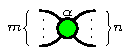
\includegraphics{generater_green_spider}
			}
			\subcaptionbox{Red spider}[2.5 cm]{%
				\centering
				
\includegraphics{generater_red_spider}
			}
			\subcaptionbox{Hadamard}[2.5 cm]{%
				\centering
				
\includegraphics[]{generater_hadamard}
			}
			\subcaptionbox{Diamond}[2 cm]{%
				\centering
				
\includegraphics{generater_diamond}
			}
			%%%%%%%%%%%%%%%%%%%%%%
		\end{minipage}
	}
	\caption{Generators for the category $\mathbf{zx}$}
	\label{fig:ZX generators}
\end{figure}
These can be combined in various ways to form larger, more complex diagrams.   Observe that these diagrams have dangling wires on the left and right. Think of those on the left as inputs and those on the right as outputs.  Formalizing this perspective, we let these diagrams generate the morphisms of a dagger compact category $\mathbf{zx}$ whose objects are the non-negative integers, the meaning of which is number of inputs and outputs.  Section \ref{sec:ZxCalc} contains a presentation of $\mathbf{zx}$ along with a brief discussion of the origins of the generating morphisms (Figure \ref{fig:ZX generators}) and generating relations (Figure \ref{fig:ZX equations}). This is a merely a brief primer and contains nothing new.  There, we also mention software tools Quantomatic \cite{BarKissingerVicary_Globular,DixonDuncanKissinger_QuantomaticWebsite} and Globular \cite{BarKissingerVicary_Globular} that are used to compute with the types of diagrams found in the zx-calculus.  

Our goal in this paper is to introduce a symmetric monoidal and compact closed (SMCC) bicategory $\underline{\mathbf{zx}}$ that categorifies $\mathbf{zx}$ in the sense that the $1$-cells of $\underline{\mathbf{zx}}$ will correspond to the zx-diagrams.  Building this correspondence, however, requires a bit of labor. We begin Section \ref{sec:RewritingOpenGraphs} by discussing open graphs and starting construction on a bicategory that suitably houses these open graphs.  With this in mind, we slightly modify past work of the author and Courser \cite{Cicala_SpansCospans, CicalaCourser_BicatSpansCospan} to produce an SMCC-bicategory with graphs as $0$-cells, cospans of graphs as $1$-cells, and certain isomorphism classes of spans of cospans (see Figure \ref{fig:spans of cospans}) of graphs as $2$-cells.   
\begin{figure}
	\fbox{%
		\begin{minipage}{\textwidth}
			\centering
			%%%%%%%%%%%%%%%%%%%%%%%%%%%%%%%
			\subcaptionbox{A span of cospans}[5cm]{%
				\centering				
				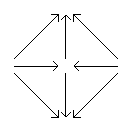
\includegraphics{diagram_span_cospans}
			}
			\subcaptionbox{A span of cospans morphism}[5cm]{%
				\centering
				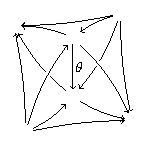
\includegraphics{scC+Map_of_Spans_of_Cospans}
			}
			%%%%%%%%%%%%%%%%%%%%%%%%%%%%%%%%
		\end{minipage}
	}
	\caption{A generic $2$-cell in $\mathbf{Sp}(\mathbf{Csp}(C))$}
	\label{fig:spans of cospans}
\end{figure}
This has a $1$-full and $2$-full sub-bicategory $\mathbf{Rewrite}$ consisting of non-negative integers as $0$-cells, open graphs as $1$-cells, and rewrite rules of open graphs as $2$-cells.  The SMCC bicategory $\mathbf{Rewrite}$ is a nice ambient space in which to generate systems modeled on open graphs.  In this paper, we exploit $\mathbf{Rewrite}$ to model the zx-calculus.

In Section \ref{sec:OpenGraphsOverSzx}, we discuss \emph{open graphs over $S_{\text{zx}}$}.  That is, we pick a graph $S_{\text{zx}}$
\[
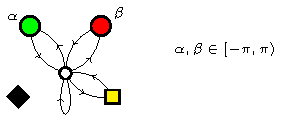
\includegraphics{graph_S_zx}
\]  
in such a way that graph morphisms $G \to S_{\text{zx}}$ correspond exactly to the zx-morphisms.  These form an SMCC bicategory with graphs over $S_{\text{zx}}$ as $0$-cells, cospans of graphs over $S_{\text{zx}}$ as $1$-cells, and certain isomorphism classes of spans of these cospans as $2$-cells.  This contains a sub-bicategory named $\mathbf{zxRewrite}$ that is analogous to $\mathbf{Rewrite}$. Though to define $\mathbf{zxRewrite}$, we first introduce the functor $N_{\text{zx}} \colon \mathbf{Set}_0 \to \left(\mathbf{Graph} \downarrow S_{\text{zx}} \right)$ from a skeleton $\mathbf{Set}_0$ of the category of sets to the slice category $\mathbf{Graph} \downarrow S_{\text{zx}}$ of graphs over $S_{\text{zx}}$ .  Define $N_{\text{zx}}(X)$ to be the edgeless graph with nodes $X$ and is constant on the $S_{\text{zx}}$-node $\begin{tikzpicture} \node [zxopen] at (0,0) {}; \end{tikzpicture}$.  Then $\mathbf{zxRewrite}$ is defined to be $1$-full and $2$-full on the $0$-cells of form $N_{\text{zx}} (X)$.  

Now, $\mathbf{zxRewrite}$ is a space in which we can generate SMCC sub-bicategories. In Section \ref{sec:zx categorified}, we give a presentation for a sub-bicategory $\underline{\mathbf{zx}}$ of $\mathbf{zxRewrite}$ by choosing $1$-cells corresponding to $\mathbf{zx}$-morphisms and $2$-cells corresponding to the relations between them.  After constructing $\underline{\mathbf{zx}}$, we decategorify it to a $1$-category $\operatorname{decat}(\underline{\mathbf{zx}})$ by identifying $1$-cells whenever there is a $2$-cell between them.  Though this identification seems asymmetrical, the dual nature of spans allows this to actually give an equivalence relation, not merely generate one.  Our main result is Theorem \ref{thm:equiv of zx cats}, in which we construct a dagger compact functor $\operatorname{decat}(\underline{\mathbf{zx}}) \to \mathbf{zx}$ that is an equivalence of categories.  

The author would like to thank his advisor John Baez for many helpful ideas and discussions that contributed to this paper.   
 
%%%%%%%%%%%%%%%%%%
%%%%%%%%%%%%%%%%%%
% 
\end{document}
%
%%%%%%%%%%%%%%%%%%
%%%%%%%%%%%%%%%%%%